%%
%% Copyright 2007-2020 Elsevier Ltd
%%
%% This file is part of the 'Elsarticle Bundle'.
%% ---------------------------------------------
%%
%% It may be distributed under the conditions of the LaTeX Project Public
%% License, either version 1.2 of this license or (at your option) any
%% later version.  The latest version of this license is in
%%    http://www.latex-project.org/lppl.txt
%% and version 1.2 or later is part of all distributions of LaTeX
%% version 1999/12/01 or later.
%%
%% The list of all files belonging to the 'Elsarticle Bundle' is
%% given in the file `manifest.txt'.
%%

%% Template article for Elsevier's document class `elsarticle'
%% with numbered style bibliographic references
%% SP 2008/03/01
%%
%%
%%
%% $Id: elsarticle-template-num.tex 190 2020-11-23 11:12:32Z rishi $
%%
%%
\documentclass[preprint,12pt]{elsarticle}

%% Use the option review to obtain double line spacing
%% \documentclass[authoryear,preprint,review,12pt]{elsarticle}

%% Use the options 1p,twocolumn; 3p; 3p,twocolumn; 5p; or 5p,twocolumn
%% for a journal layout:
%% \documentclass[final,1p,times]{elsarticle}
%% \documentclass[final,1p,times,twocolumn]{elsarticle}
%% \documentclass[final,3p,times]{elsarticle}
%% \documentclass[final,3p,times,twocolumn]{elsarticle}
%% \documentclass[final,5p,times]{elsarticle}
%% \documentclass[final,5p,times,twocolumn]{elsarticle}

%% For including figures, graphicx.sty has been loaded in
%% elsarticle.cls. If you prefer to use the old commands
%% please give \usepackage{epsfig}

%% The amssymb package provides various useful mathematical symbols
\usepackage{amssymb}
%% The amsthm package provides extended theorem environments
%% \usepackage{amsthm}
%% The amsmath package provides a handful of options for displaying equations.
\usepackage{amsmath}

%% The lineno packages adds line numbers. Start line numbering with
%% \begin{linenumbers}, end it with \end{linenumbers}. Or switch it on
%% for the whole article with \linenumbers.
\usepackage{lineno}

% \journal{Physics Letters A}

\usepackage[utf8]{inputenc}
\usepackage[T2A]{fontenc}
\usepackage[russian]{babel}

\begin{document}

\begin{frontmatter}

%% Title, authors and addresses

%% use the tnoteref command within \title for footnotes;
%% use the tnotetext command for theassociated footnote;
%% use the fnref command within \author or \address for footnotes;
%% use the fntext command for theassociated footnote;
%% use the corref command within \author for corresponding author footnotes;
%% use the cortext command for theassociated footnote;
%% use the ead command for the email address,
%% and the form \ead[url] for the home page:
%% \title{Title\tnoteref{label1}}
%% \tnotetext[label1]{}
%% \author{Name\corref{cor1}\fnref{label2}}
%% \ead{email address}
%% \ead[url]{home page}
%% \fntext[label2]{}
%% \cortext[cor1]{}
%% \affiliation{organization={},
%%             addressline={},
%%             city={},
%%             postcode={},
%%             state={},
%%             country={}}
%% \fntext[label3]{}

\title{Многоквантовый ЯМР в твердых телах как метод определения информации Вигнера--Янасе}

%% use optional labels to link authors explicitly to addresses:
%% \author[label1,label2]{}
%% \affiliation[label1]{organization={},
%%             addressline={},
%%             city={},
%%             postcode={},
%%             state={},
%%             country={}}
%%
%% \affiliation[label2]{organization={},
%%             addressline={},
%%             city={},
%%             postcode={},
%%             state={},
%%             country={}}




\author[icp]{C.~И.~Доронин}
\author[icp]{Э.~Б.~Фельдман}
\author[icp,msu]{И.~Д.~Лазарев}
\address[icp]{Институт проблем химической физики Российской Академии Наук, \\ Черноголовка, Москва, Россия 142432} 
\address[msu]{Факультет фундаментальной физико-химической инженерии. МГУ им. Ломоносова, GSP-1, Москва. Россия 119991}

\begin{abstract}
%% Text of abstract
В многоквантовом эксперименте  (МК) ЯМР в твердых телах рассматривается связь косой информации Вигнера--Янасе и  МК когерентностей ЯМР при разных температурах и временах эволюции ядерных спинов с диполь-дипольными взаимодействиями.
Показано, что косая информация Вигнера--Янасе при температуре $T$ равна удвоенному второму моменту  спектра МК когерентностей ЯМР  при температуре $2T$ для любых времен эволюции.
Проводится сравнение оценок многочастичной запутанности, полученной с помощью косой информации Вигнера--Янасе и информации Фишера.
\end{abstract}

%%Graphical abstract
%\begin{graphicalabstract}
%\includegraphics{...}
%\end{graphicalabstract}

%%Research highlights
% \begin{highlights}
% 	\item multiple quantum NMR spectroscopy
% 	\item connection between the Wigner-Yanase skew information and the second moment of the distribution of multiple quantum coherences
% 	\item the dependence of the number of entangled spins on temperature
% \end{highlights}

\begin{keyword}
%% keywords here, in the form: keyword \sep keyword
    многочастичная запутанность \sep
    информация Фишера \sep
    косая информация Фишера \sep
    многоквантовый ЯМР \sep
    многоквантовые когерентности \sep
    второй момент \sep
    температура
    
%% PACS codes here, in the form: \PACS code \sep code
%\PACS 0000 \sep 1111
%%
%% MSC codes here, in the form: \MSC code \sep code
%% or \MSC[2008] code \sep code (2000 is the default)
%\MSC 0000 \sep 1111
\end{keyword}

\end{frontmatter}

% \linenumbers

%% main text

\section{Introduction}
\label{sec:1}
Косая информация Вигнера--Янасе~\cite{1,2,3,4} так же, как и информация Фишера~\cite{5,6} позволяет разрабатывать методы для исследования многочастичной запутанности~\cite{7,8}. 
Дальнейшее исследование многочастичной запутанности требует разработки соответствующих экспериментальных методов.
В частности, было показано~\cite{7,9}, что нижняя граница квантовой информации Фишера~\cite{5,6} совпадает со вторым моментом спектра многоквантовых (МК) когерентностей. 
В результате нижняя граница квантовой информации Фишера может быть найдена в МК эксперименте ЯМР~\cite{10},
в экспериментах с холодными атомами, включая эксперименты с Бозе-Эйнштейновскими конденсатами, ионами в ловушках и др.~\cite{11,12,13,14,15}. 
Используя свойства квантовой информации Фишера можно получить оценку снизу для числа запутанных частиц (спинов) в рассматриваемой системе~\cite{7} и даже найти зависимость этой оценки от температуры~\cite{9}. 


Косая информация Вигнера-Янасе~\cite{1,2,3,4} также связана со спектром МК когерентностей. 
В частности в данной работе мы демонстрируем, 
что косая информация Вигнера--Янасе в системе спинов $(s = 1/2)$ c диполь-дипольным взаимодействием (ДДВ) в МК эксперименте ЯМР~\cite{10} с температурой системы $T$ 
равна второму моменту спектра МК когерентностей ЯМР полученном при температуре $2T$. 
Используя это свойство косой информации Вигнера--Янасе можно исследовать многочастичную запутанность на базе МК спектроскопии ЯМР~\cite{10}.


Главная цель данной работы это разработка метода извлечения косой информации Вигнера--Янасе из спектра МК когерентностей ЯМР. 
Мы также провели сравнение оценок многочастичной запутанности, полученных с помощью косой информации Вигнера--Янасе и информации Фишера для простой модели~\cite{8,16}.  



\section{МК ЯМР для решения проблем квантовой информатики}
\label{sec:2}


\begin{figure}
	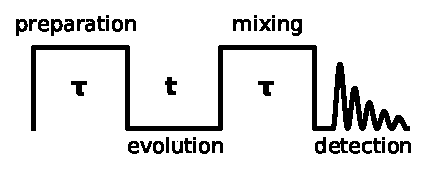
\includegraphics[width=0.95\linewidth]{mq-experiment}
	\caption{Схема многоквантового эксперимента ЯМР.}
	\label{fig:1}
\end{figure}

Методы МК ЯМР широко используются для решения проблем квантовой информатики~\cite{17,18}. 
МК эксперимент ЯМР состоит из четырех уникальных периодов времени, изображенных на рисунке Рис.~\ref{fig:1}:
подготовительный период $(\tau)$, период свободной эволюции $(t_1)$, период смешивания $(\tau)$ и период детектирования $(t_2)$~\cite{10}.
МК когерентности ЯМР создаются периодической многоимпульсной последовательностью, 
состоящей из $\pm$x-импульсов, которой облучают систему на подготовительном периоде~\cite{10}.
Если период обращенной многоимпульсной последовательности значительно превышает локальное дипольное поле (в частотных единицах)~\cite{19}, 
тогда МК динамика ЯМР может быть описана усредненным несекулярным двухквантовым Гамильтонианом~$H_{MQ}$~\cite{20}. 
%
\begin{equation} \label{eq:1}
        H_{MQ} = H^{(+2)} + H^{(-2)} , \quad
        H^{(\pm 2)} = -\frac{1}{2} \sum_{j<k} D_{jk} I_{j} ^\pm I_k^\pm,
\end{equation}
%
где $D_{jk}$ это константа диполь-дипольного взаимодействия между спинами $j$ и $k$,
а $I_{j}^+, I_k ^-$ это повышающий и понижающий операторы для спина $j$.
На периоде смешивания спиновая система облучается многоимпульсной последовательностью $\pm y$--импульсами. 
В результате средний несекулярный двухквантовый Гамильтониан  на периоде смешивания равен~$(-H_{MQ})$~\cite{10}.


В частности, для исследования МК динамики ЯМР для системы на подготовительном периоде~\cite{10} 
следует найти матрицу плотности $\rho(t)$, решив эволюционное уравнение Лиувилля~\cite{19}. 

\begin{equation}
    \label{eq:2}
        i\frac{d\rho(t)}{dt} = [H_{MQ}, \rho(t)]
\end{equation}
С начальным термодинамически равновесным состоянием
\begin{equation}
    \label{eq:3}
        \rho(0) = \rho_\mathrm{eq} = \frac{\exp(\frac{\hbar \omega_0}{kT}I_z)}{Z},
\end{equation}
где $Z=Tr \left\{exp\left(\frac{\hbar \omega_0}{kT}I_z\right) \right\}$ это статистическая сумма,
$\hbar$ и $k$ это постоянные Планка и Больцмана соответственно,
$\omega_0$ это Ларморовская частота, 
$T$ - это температура
и $I_z$ - это оператор проекции полного углового момента на ось~$z$,
которая направлена вдоль сильного внешнего магнитного поля. 


Объединяя подготовительный период, период эволюции и период смешивания, 
а также взяв во внимание инкремент фазы $\phi$ радиочастотных импульсов~\cite{10}, 
результирующий сигнал $G(\tau,\phi)$ хранится в виде информации о населенности
%
\begin{equation} \label{eq:4}
	\begin{split}
		G(\tau,\phi)
		& = Tr \left\{
			e^{iH_{MQ}\tau} e^{i\phi I_z} e^{-iH_{MQ}\tau} \rho_\mathrm{eq}
			e^{iH_{MQ}\tau} e^{-i\phi I_z} e^{-iH_{MQ}\tau}\rho_\mathrm{eq}
		\right\}
		\\
		& = Tr \left\{
			e^{i\phi I_z} \rho_\mathrm{pre}(\tau,\beta)
      e^{-i\phi I_z}\rho_\mathrm{pre}(\tau,\beta)
		\right\},
	\end{split}
\end{equation}
%
где
%
\begin{equation} \label{eq:5}
	\rho_\mathrm{pre}(\tau,\beta) = e^{-iH_{MQ}\tau}\rho_\mathrm{eq}e^{iH_{MQ}\tau}
\end{equation}
%
это матрица плотности в конце подготовительного периода. 
Матрица плотности может быть получена из Ур.~(\ref{eq:2},\ref{eq:3}) и $\beta = \frac{\hbar \omega_0}{kT}$.


Удобно представить матрицу плотности~$\rho_\mathrm{pre}(\tau, \beta)$ в виде ряда~\cite{21}
\begin{equation}
    \label{eq:6}
        \rho_\mathrm{pre}(\tau,\beta) = \sum_n \rho_{\mathrm{pre},n}(\tau,\beta),
\end{equation}
где $\rho_{\mathrm{pre}, n}(\tau,\beta)$ это вклад МК когерентности n--ого порядка в матрицу плотности $\rho_\mathrm{pre}(\tau,\beta)$.  
Тогда результирующий сигнал~$G(\tau,\phi)$ МК ЯМР~\cite{10} можно переписать в виде 
\begin{equation} \label{eq:7}
    G(\tau, \phi) = \sum_n e^{in\phi}
        Tr\left\{\rho_{\mathrm{pre},n}(\tau,\beta)
        \rho_{\mathrm{pre},-n}(\tau,\beta) \right\},
\end{equation}
где мы берем во внимание, что 
\begin{equation}
    \label{eq:8}
        [I_z, \rho_{\mathrm{pre},n}] = n \rho_{\mathrm{pre},n}
\end{equation}
Нормализованные интенсивности МК когерентностей ЯМР могут быть определены как
\begin{equation}
    \label{eq:9}
        J_n(\tau,\beta)= \frac{Tr\left\{\rho_{\mathrm{pre},n}(\tau,\beta)
            \rho_{\mathrm{pre},-n}(\tau,\beta)\right\}}
                {Tr(\rho^2_\mathrm{eq})}
\end{equation}
Как было паказано в~\cite{8},
\begin{equation}
    \label{eq:10}
        Tr(\rho_\mathrm{eq}^2) = \frac{2^N ch^N (\beta)}{Z^2},
\end{equation}
где $N$ это число спинов в спиновой системе. 
Также было показано, что 
\begin{equation}
    \label{eq:11}
        \sum_n J_n(\tau,\beta) = 1
\end{equation}
Второй момент (дисперсия) $M_2(\tau,\beta)$ распределения интенсивностей МК когерентностей ЯМР  $J_n (\tau,\beta)$ может быть вычислен из Ур.~(\ref{eq:7}) согласно~\cite{22}.  
\begin{equation}
    \label{eq:12}
        M_2(\tau,\beta) = -\frac{1}{G(\tau, \beta)}
            \frac{d^2 G(\tau + t,\beta)}{dt^2}\bigg|
        _{t=0}
\end{equation}
Используя Ур.~(\ref{eq:7},\ref{eq:8},\ref{eq:12}) можно получить
\begin{equation}
    \label{eq:13}
        M_2 (\tau,\beta) = \sum_n n^2 J_n(\tau,\beta)
\end{equation}
Нижняя граница квантовой информации Фишера совпадает со вторым моментом Eq.~(\ref{eq:13})~\cite{7,9}.
В результате анализ температурной зависимости второго момента $M_2(\tau,\beta)$ распределения интенсивностей МК когерентностей ЯМР позволяет нам получить оценку числа запутанных спинов для разных температур~\cite{8}.
В следующем разделе~\ref{sec:3} мы продемонстрируем, что косая информация Вигнера--Янасе
также связана со вторым моментом $M_2(\tau,\beta)$ 
и может быть полезна для исследования многочастичной запутанности. 

\section{Косая информация Вигнера--Янасе и МК ЯМР}
\label{sec:3}
Косая информация Вигнера--Янасе определяется как~\cite{1,2,3,4} 
\begin{equation}
    \label{eq:14}
        I_{WY}(\rho(\tau,\beta),I_z) = -\frac{1}{2}
            Tr([\sqrt{\rho(\tau,\beta)},\sigma_z])^2 =
                -2Tr([\sqrt{\rho(\tau,\beta)},I_z])^2,
\end{equation}
где~$\sigma_z=2I_z$~оператор Паули. 
Введем оператор эволюции
\begin{equation}
    \label{eq:15}
        V(\tau) = e^{iH_{MQ}\tau}
\end{equation}
и, используя Ур.~(\ref{eq:3}), можем записать матрицу плотности $\rho(\tau,\beta)$ как:
\begin{equation}
    \label{eq:16}
        \rho(\tau,\beta) = V^+(\tau) \frac{e^{\beta I_z}}{Z}V(\tau)
\end{equation}
Теперь мы используем очевидное соотношение:
\begin{equation}
    \label{eq:17}
        \sqrt{\rho(\tau,\beta)} =
            \sqrt{V^+(\tau)\frac{e^{\beta I_z}}{Z}V(\tau)} =
                V^+(\tau) \frac{e^{\frac{\beta}{2}I_z}}{\sqrt{Z}}V(\tau).
\end{equation}
Это можно доказать простым вычислением:
\begin{equation}
    \label{eq:18}
        \sqrt{\rho}\sqrt{\rho} =
						V^+(\tau)\frac{e^{\frac{\beta}{2}I_z}}{\sqrt{Z}}
                V(\tau)V^+(\tau)\frac{e^{\frac{\beta}{2}I_z}}{\sqrt{Z}}V(\tau) =
						V^+(\tau)\frac{e^{\beta I_z}}{Z}V(\tau) =
        \rho(\tau,\beta)
\end{equation}
%
Теперь мы получаем
%
\begin{equation} \label{eq:19}
    \left[I_z,\sqrt{\rho(\tau,\beta)}\right]
    = \left[I_z, \sum_k \rho_k \left(\tau, \frac{\beta}{2}\right)\right]
    = \sum_k k\rho_k \left(\tau, \frac{\beta}{2}\right),
\end{equation}
%
и
%
\begin{equation} \label{eq:20}
	Tr\left[I_z,\sqrt{\rho(\tau,\beta)} \right]^2
	= Tr\left\{\sum_{k,k'}kk'
		\rho_k\left(\tau,\frac{\beta}{2}\right)
		\rho_{k'}\left(\tau,\frac{\beta}{2}\right)
	\right\}
	= \sum_k k^2 J_k\left(\tau,\frac{\beta}{2}\right).
\end{equation}
%
В итоге мы получаем, что
%
\begin{equation} \label{eq:21}
    I_{WY}\left(\rho(\tau, \beta), I_z\right)
    = 2\sum_k k^2 J_k\left(\tau, \frac{\beta}{2}\right)
    = 2M_2\left(\tau, \frac{\beta}{2}\right)
\end{equation}
%
Таким образом мы получили важное наблюдение.
Если спиновая система исследуется с помощью МК ЯМР при температуре $T\sim\beta^{-1}$
тогда косая информация Вигнера--Янасе равна второму моменту распределения интенсивности МК когерентностей ЯМР при температуре $2T \sim 2\beta^{-1}$ для любого времени эволюции. 


Косая информация Вигнера--Янасе связана со вторым моментом распределения интенсивности МК когерентностей ЯМР так же как и информация Фишера.
Сравнение оценок многочастичной запутанности на основе этих информаций приведено в следующей секции~\ref{sec:4}. 



\section{Сравнение оценок многочастичной запутанности, полученной с помощью косой информации Вигнера--Янасе и информации Фишера}
\label{sec:4}

\begin{figure}
	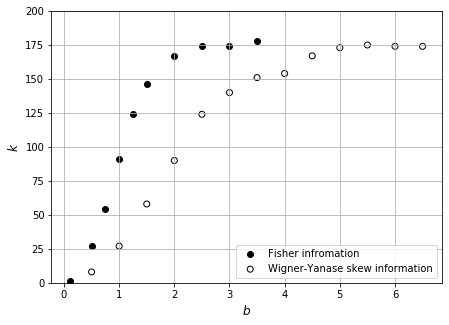
\includegraphics[width=0.95\linewidth]{nanopora_entangled_spins_by_temp}
	\caption{
	    Зависимость $N_\mathrm{ent}$ оценки снизу для числа запутанных спинов от обратной температуры $\beta = \frac{\pi \omega_0}{kT}$ для системы эквивалентных спинов;
	    черные точки --- результаты полученные из информации Фишера;
	    белые точки --- результаты полученные из косой информации Вигнера--Янасе;
	}
	\label{fig:2}
\end{figure}

\begin{figure}
	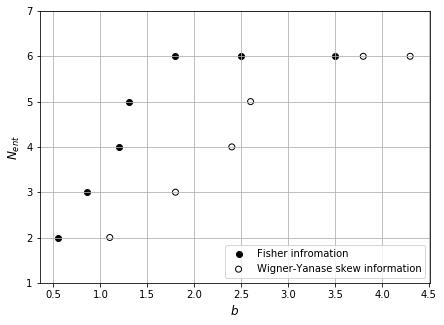
\includegraphics[width=0.95\linewidth]{zigzag_entangled_spins_by_temp}
	\caption{
	    Зависимость $N_\mathrm{ent}$ оценки снизу для числа запутанных спинов от обратной температуры $\beta = \frac{\pi \omega_0}{kT}$ для альтерированной  цепочки;
	    черные точки --- результаты полученные из информации Фишера;
	    белые точки --- результаты полученные из косой информации Вигнера--Янасе;
	}
	\label{fig:3}
\end{figure}

Косая информация Фишера  $I_{WY}(\rho(\tau,\beta),I_z)$ и информация Фишера $I_F(\rho(\tau,\beta),I_z)$
могут быть использованы для исследования многочастичной запутанности. 
Известно~\cite{5,6}, что если
$I_{WY}\left( \rho(\tau, \beta), I_z \right)$
или
$I_{F}\left( \rho(\tau, \beta), I_z \right)$
превышает $mk^2 + (N - mk)^2$,
где $k, m$ целые, а $m$ это целая часть от $N/k$,
тогда состояние содержит несепарабельную подсистему с $N_\mathrm{ent} = (k + 1) $ частицами. 
Информации связанны следующим неравенством~\cite{3}:
%
\begin{equation} \label{eq:22}
    I_{WY}\left(\rho(\tau,\beta), I_z\right)
    \leq I_F\left(\rho(\tau,\beta), I_z\right)
    \leq 2I_{WY}\left(\rho(\tau,\beta), I_z\right).
\end{equation}
%
Данное неравенство~(\ref{eq:22}) позволяет нам надеяться, что результаты для оценки количества запутанных спинов не будут значительно отличаться. 
Для сравнения мы используем модель~\cite{23} несферической нанопоры, заполненной газом спин несущих атомов (например, ксенон) или молекул в сильном внешнем магнитном поле. 
Эта модель позволяет исследовать многочастичную запутанность в спиновой системе, состоящей из сотни ядерных спинов~\cite{8}. 


Мы исследуем многочастичную запутанность в спиновой системе, состоящую из 201 спина
в нанопоре. На Рис.~\ref{fig:2} изображена зависимость $N_\mathrm{ent}$ оценки снизу для числа запутанных спинов от обратной температуры. Число запутанных спинов растет с понижением температуры для обеих информаций. 

Также по аналогии было проведено исследование модели альтерированной цепочки протонов в монокристалле гамбергита~\cite{16,24}.
На Рис.~\ref{fig:3} изображен схожее поведение многочастичной запутанности для цепочки из 6 спинов для обеих информаций. 


\section{Выводы}
\label{sec:5}

Мы изучили связь косой информации Вигнера--Янасе со вторым моментом распределения интенсивностей МК когерентностей ЯМР в МК эксперименте ЯМР. 
Было параказно, что косая информация Вигнера--Янасе при температуре $T \sim \beta^{-1}$ равна 
удвоенному второму моменту МК ЯМР спектра при температуре $2T \sim 2\beta^{-1}$.
Было проведено сравнение оценок количества запутанных спинов полученных с помощью косой информации Вигнера--Янасе и информации Фишера.


\section{Acknowledgement}
\label{sec:6}
Мы благодарим фонд Министерства науки и высшего образования РФ (Grant No.~075-15-2020-779)





%% The Appendices part is started with the command \appendix;
%% appendix sections are then done as normal sections
%\appendix
%\section{Sample Appendix Section}
%\label{sec:sample:appendix}
%Lorem ipsum dolor sit amet...

%% If you have bibdatabase file and want bibtex to generate the
%% bibitems, please use
%%
% \bibliographystyle{elsarticle-num}
% \bibliography{bibliography}

%% else use the following coding to input the bibitems directly in the
%% TeX file.

% \begin{thebibliography}{00}

% %% \bibitem{label}
% %% Text of bibliographic item

% \bibitem{}

% \end{thebibliography}

\begin{thebibliography}{20}
  \bibitem{1} E.P.Wigner, M.M. Yanase, Proc.Nat.Acad.Sei. USA \textbf{49}, 910-918 (1963)
  \bibitem{2} S.Luo, Phys.Rev.Lett. \textbf{91}, 180403 (2003)
  \bibitem{3} S.Luo, Proc.Amer. Math.Soc. \textbf{132}, No.885-890 (2003)
  \bibitem{4} Z.Chen, Phys.Rev. A \textbf{71}, 052302 (2005)
  \bibitem{5} G.Toth, I.Apellaniz, J. Phys. A \textbf{47},424006 (2014)
  \bibitem{6} L.Pezze, A.Smerzi, M.K. Oberthaler, R. Schmied, P.Treutlein, Rev.Mod.Phys. \textbf{90}, 035005 (2018)
  \bibitem{7} M.Gartner, P.Hauke, A.M.Rey, Phys.Rev.Lett. \textbf{120}, 040402 (2018)
  \bibitem{8} S.I.Doronin, E.B.Fel'dman, I.D.Lazarev, Phys. Rev. A \textbf{100},022330 (2019)
  \bibitem{9} D.Girolami, B.Yadin,Entropy \textbf{19},124 (2017)
  \bibitem{10} J.Baum, M.Munowitz, A.N.Garroway, A.Pines,J.Chem.Phys. \textbf{83}, 2015 (1985)
  \bibitem{11} B. Swingle, G. Bentsen, M. Scheleier-Smith, P. Hayden, Phys.	Rev. A \textbf{94}, 040302 (2010)
  \bibitem{12} F.M. Cucchietti, J.Opt.Soc. Am. B\textbf{27}, A30 (2010)
  \bibitem{13} I.D. Leroux, M.H. Schleier-Smith, V.Vuletic, Phys.Rev.Lett. \textbf{104}, 073602 (2010)
  \bibitem{14} T.Macri, A. Smerzi, L.Pezze, Phys.Rev. A \textbf{94}, 010102 (2016)
  \bibitem{15} M.Gartner, J.G.Bohnet, A.Safavi-Naini, M.L. Wall, J.J. Bollinger, A.M.Rey, Nat.Phys. \textbf{13} ,781 (2017)
  \bibitem{16} G.A.Bochkin, S.G.Vasil'ev, S.I. Doronin, E.I.Kuznetsova,I.D.Lazarev,E.B.Fel'dman, Appl.Magn.Reson. \textbf{51},667-678 (2020)
  \bibitem{17} E.B.Fel'dman, A.N. Pyrkov, A.I.Zenchuk, Philos. Trans. R. Soc. London A\textbf{370}, 4690 (2012)
  \bibitem{18} G.B.Furman, V.M.Meerovich, V.L.Sokolovsky, Phys. Rev. A \textbf{78} 042301 (2008)
  \bibitem{19} M.Goldman. Spin temperature and nuclear magnetic resonance in solids, Oxford,UK, Clarendon Press. 1970.
  \bibitem{20} S.I.Doronin, I.I.Maksimov, E.B.Fel’dman, J. Exp. Theor. Phys.\textbf{91}, 597 (2000)
  \bibitem{21} E.B.Fel'dman, S.Lacelle,Chem.Phys.Lett. \textbf{253}, 27 (1996)
  \bibitem{22} A.Abragam, The Principles of Nuclear Magnetism, Clarendon. Oxford. 1961
  \bibitem{23} J. Baugh, A. Kleinhammes, D. Han, Q. Wang, Y.Wu, Science \textbf{294}, 1505 (2001)
  \bibitem{24} G.A. Bochkin, E.B. Fel'dman, E.B. Kuznetsova, I.D. Lasarev, S.G. Vasil'ev, V.I.Volkov, J. Magn.Reson. \textbf{319}, 106816 (2020)
\end{thebibliography}

\end{document}
\endinput
